\documentclass{beamer}
\usetheme{boadilla}


\usepackage{amsmath,amssymb,amsthm} 
\usepackage{caption}
\usepackage{gensymb}
\usepackage{preview}
\usepackage{bm}
\usepackage{mathtools}
\usepackage{hyperref} 
\usepackage{fancyhdr}
\usepackage{indentfirst}
\usepackage{tablefootnote}
%\usepackage{cmbright}
\usepackage[russian, english]{babel}
\usepackage[T1,T2A]{fontenc}
\usepackage[utf8]{inputenc}
\usepackage [autostyle, english = american]{csquotes}
\MakeOuterQuote{"}

\title{Clustering, Mixtures, and the EM Algorithm}
\subtitle{Machine Learning: Module 1}
\author{Sean Norton; Simon Hoellerbauer}
\begin{document}
\begin{frame}
	\titlepage
\end{frame}

\section{Cluster Analysis}

\begin{frame}
\frametitle{The Problem: Finding Groups}
	In social science, we often believe our observations have some sort of group structure.
	\begin{itemize}
		\item Regime types
		\item Types of voters
		\item Types of legislators		
	\end{itemize}
	However, our data doesn't (generally) come with these groupings conveniently pre-labeled.

\end{frame}

\begin{frame}
\frametitle{E.g. Regime Types}
	
	\begin{figure}
		\centering
		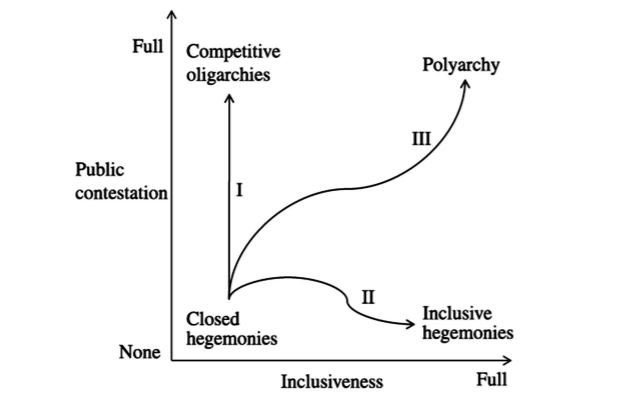
\includegraphics[width=0.7\linewidth]{dahl}
		\caption{Dahl: Regime Types}
		\label{fig:dahl}
	\end{figure}

\end{frame}

\begin{frame}
\frametitle{The Problem Continued}
	The general approach to dealing with this problem has been to hand-label cases. This is problematic because:
	\begin{itemize}
		\item It's time-consuming
		\item Humans aren't able to consider all available data at once
		\item It relies on researcher discretion
		\item For large datasets (e.g. all countries in the world), this is impossible.
	\end{itemize}
	What if there was a way to find latent groupings between our cases quickly and with as little researcher discretion as possible?
\end{frame}

\begin{frame}
\frametitle{Enter Cluster Analysis}
	This is exactly what cluster analysis is intended to do!\\
	Given:
	\begin{itemize}
		\item Data
		\item Number of clusters
		\item Variables
		\item Similarity measure
	\end{itemize}
	A cluster analysis algorithm finds groupings, or clusters, that maximize the similarity between observations within a cluster. 
\end{frame}

\begin{frame}
\frametitle{K-Means and Notation}
	One of the most common similarity measures is the squared distance between the center (mean) of a cluster. \\
	This is known as \textit{k-means} or \textit{k-nearest neighbor} clustering.\\
	Before we dive into the math, some notation:
	\begin{itemize}
		\item $k$: total number of clusters
		\item $r_{nk}$: indicator vector of cluster membership for observation $x_n$
		\item $\mu_k$: the centroid of cluster $k$
	\end{itemize}
\end{frame}

\begin{frame}
\frametitle{K-Means: The Math}
	Cluster analysis relies on a measure of similarity, which in k-means is:
	
	\begin{align*}
	J = \sum_{n=1}^{N}\sum_{k=1}^{K} r_{nk}  \| x_n - \mu_k \|^2
	\end{align*}
	This number $J$ is also known as a \textit{distortion measure}.\\
	What (hopefully) familiar thing does this measure look like?
\end{frame}

\begin{frame}
\frametitle{The Math cont.}
	\textbf{Q}: But how do we choose values of $\mu_k$ given that we don't actually know the cluster assignments?\\
	\textbf{A}: We don't!\\
	We can find $k_m$ through a version of the \textit{expectation-maximization algorithm}:
	\begin{enumerate}
		\item Initialize some random values for $\mu_k$
		\item Minimize $J$ w.r.t. $r_{nk}$; i.e. assign cluster memberships in order to minimize distortion
		\item Using the previous $r_{nk}$, minimize J w.r.t to $\mu_k$; i.e., assign new means that minimize distortion
		\item Repeat until convergence ($J$ does not change, or the change falls below some threshold)
	\end{enumerate}

\end{frame}

\begin{frame}
 \frametitle{The Math: Visualized}
 \begin{figure}
 	\centering
 	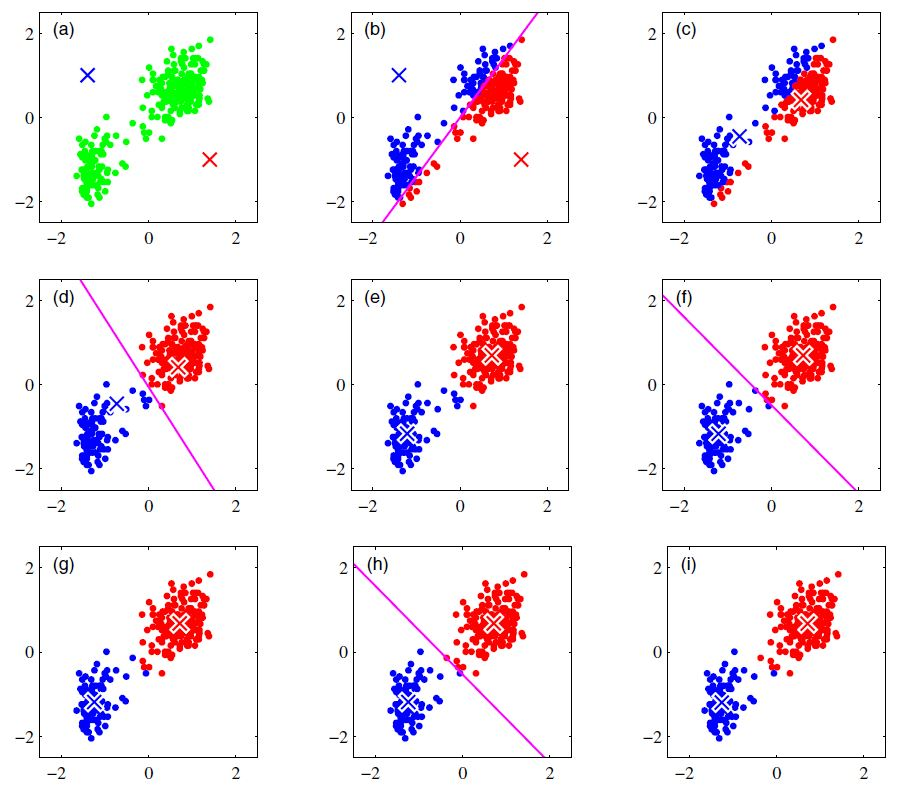
\includegraphics[width=0.7\linewidth]{bishopkmeans}
 	\caption{Optimizing Clusters}
 	\label{fig:bishopkmeans}
 \end{figure}
 
\end{frame}

\section{Clustering Problems}

\begin{frame}
	\frametitle{Problems with Clustering}
	\begin{itemize}
		\item Choosing $k$: this requires trying a lot of different $k$ w.r.t. some similarity measure
			\begin{itemize}
				\item Plot the WCSS against the number of clusters, and look for a "bend" in the plot; this is known as the elbow method
				\item Use average silhouette width: the silhouette is a measure how similar an observation is to its own cluster (consistency) and how dissimilar it is to other clusters (separation)
				\item Gap statistics: compare multiple values of $k$ to a simulated reference distribution of datasets with clusters varying from $k=1$ to $k=max$
			\end{itemize}
		\item Sensitivity to outliers; luckily, there are clustering methods other than $k$-means
			\begin{itemize}
				\item Partitioning around medoids (PAM): uses median instead of mean
				\item Hierarchical clustering: creates a tree-based representation of the data without specifying $k$; clusters are created by "cutting" the tree.  
			\end{itemize}
		\item Fundamentally descriptive; clusters will not necessarily be the same given different data
	\end{itemize}
\end{frame}

\begin{frame}
\frametitle{Problems cont.}

\begin{figure}
	\centering
	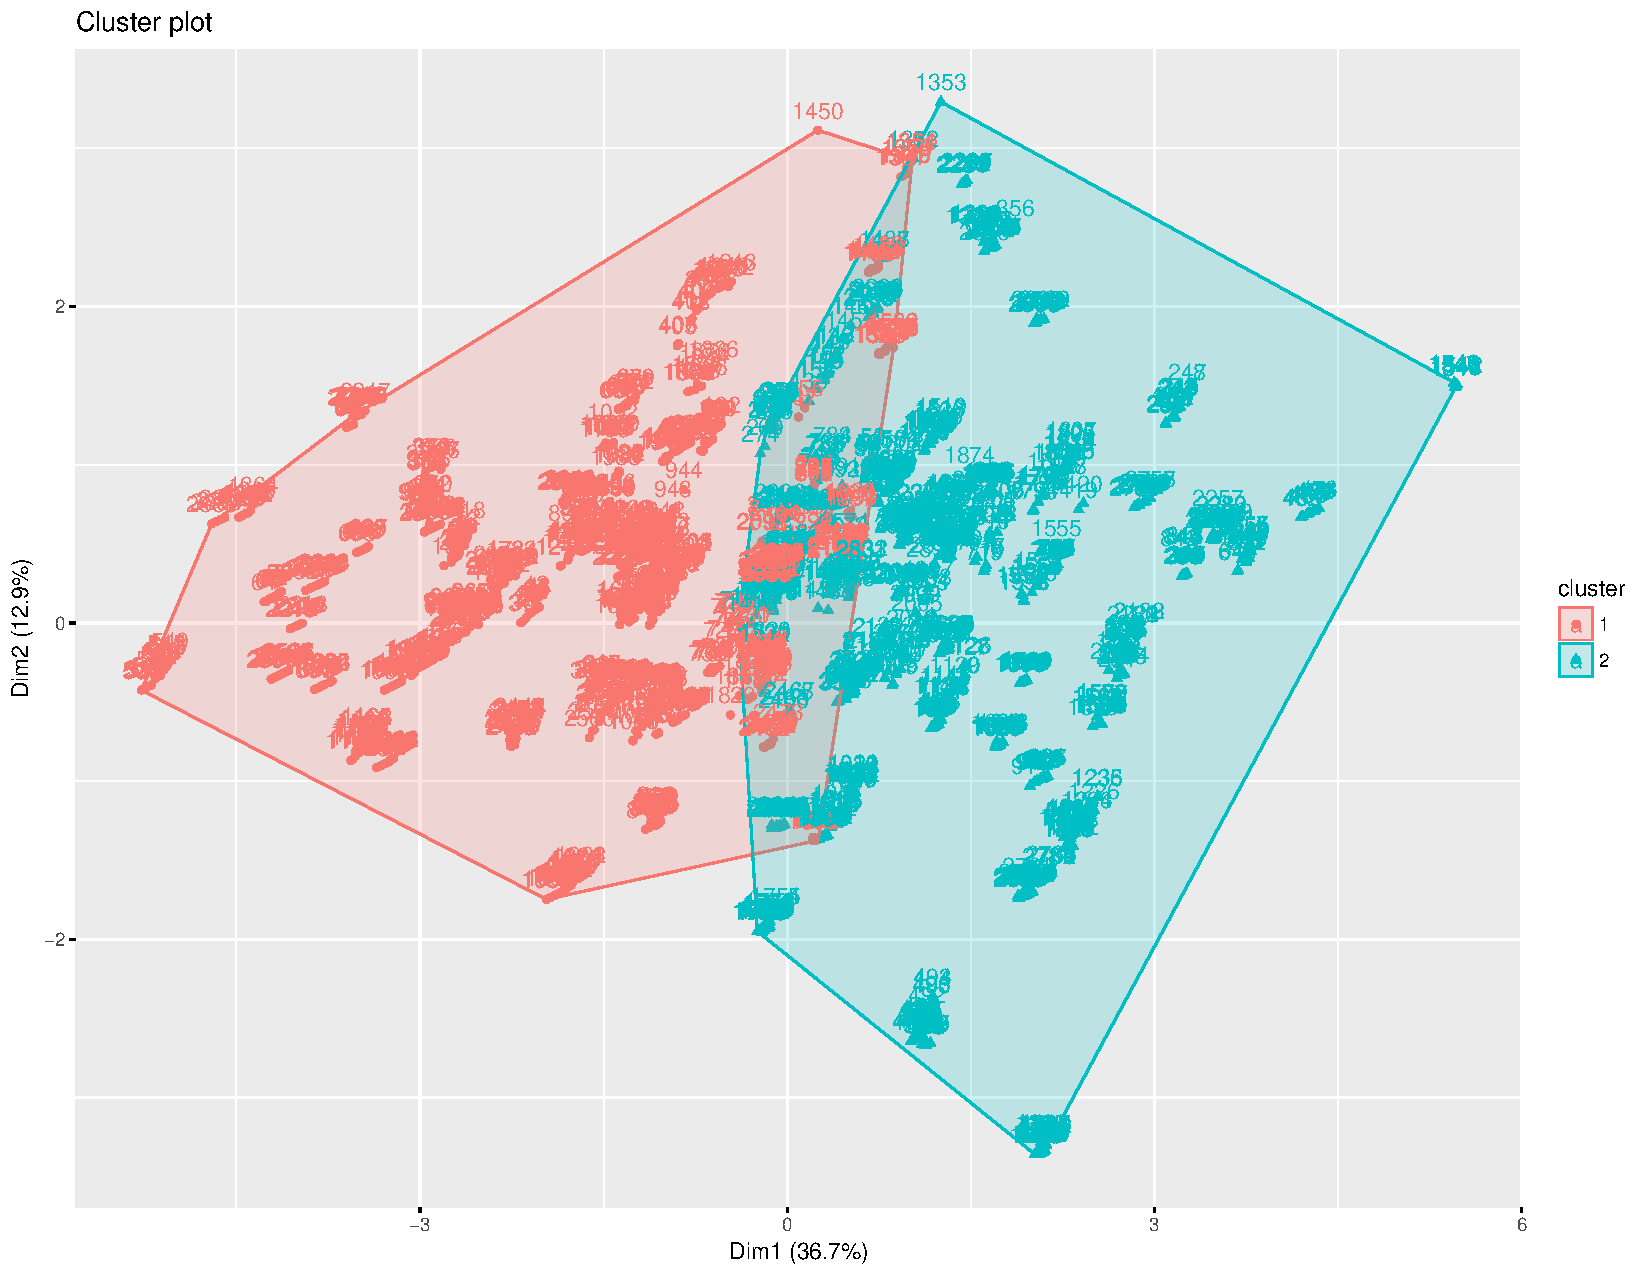
\includegraphics[width=0.7\linewidth]{clusterplot}
	\caption{My Cluster Plot}
	\label{fig:clusterplot}
\end{figure}

\end{frame}

\section{Mixture Models: Basics}

\begin{frame}
\frametitle{Mixture Models: Motivation}
	What if instead of "hard" cluster assignments, we could assign a probability that cases belong to a particular group?\\
	That is precisely what \textit{mixture models} are intended to do!\\
	Mixture models allow observations to belong to different distributions - either different parameterizations of the same distribution, or different distributions entirely.\\
	This allows us to:
	\begin{itemize}
		\item Sort cases into groups, much like cluster models, but do so in a way that quantifies uncertainty
		\item Estimate a model in the same step as the grouping, which most out-of-the-box clustering packages do not do
		\item Work with data that has a multimodal distribution without having to discard a substantial amount of variation. 
	\end{itemize}
\end{frame}

\begin{frame}
\frametitle{Motivating Example: Old Faithful}
	\begin{figure}
		\centering
		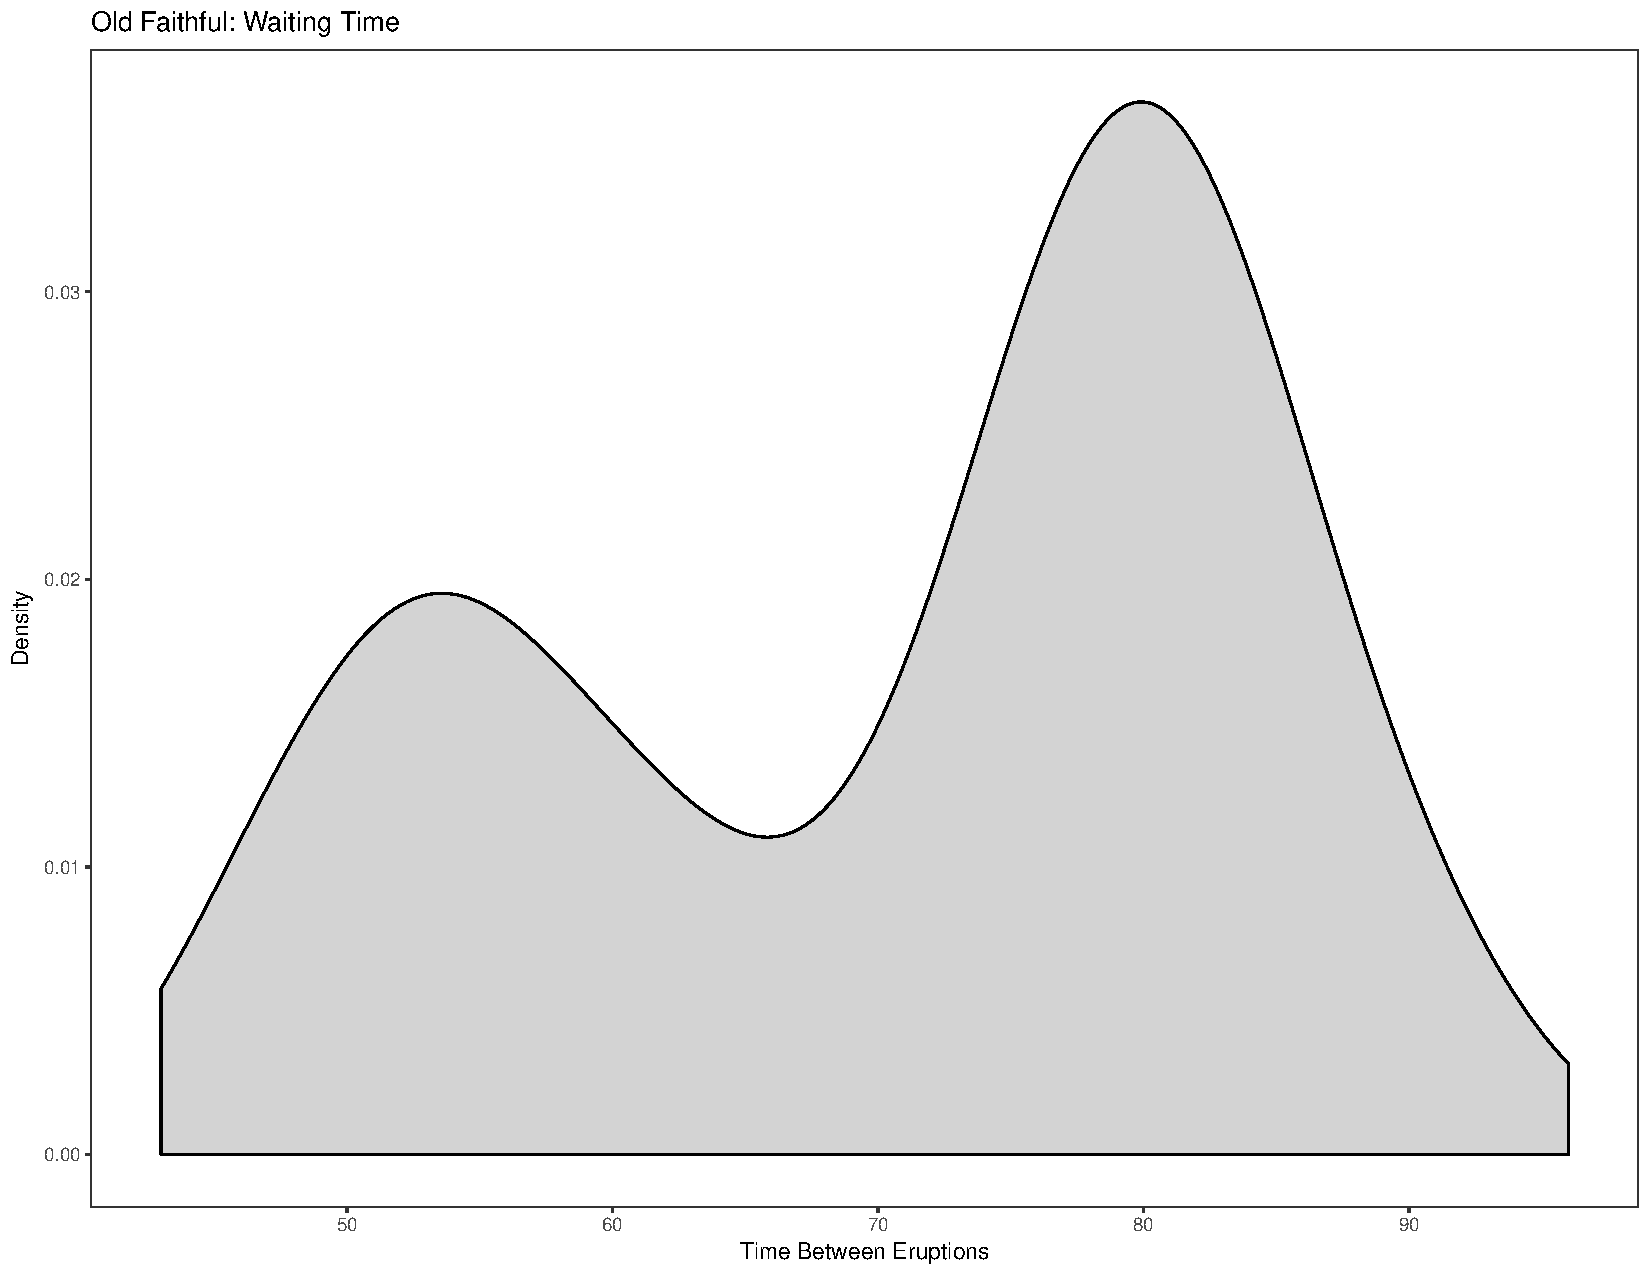
\includegraphics[width=0.7\linewidth,]{faithfulplot}
		\caption*{}
		\label{fig:faithfulplot}
	\end{figure}
	
\end{frame}

\begin{frame}
\frametitle{Motivating Example: Old Faithful}
Clearly, this data appears to be normally distributed, but not in a single normal distribution.\\
Instead of fitting a single Gaussian, we can fit a \textit{mixture} of Gaussians of the following form:
\begin{align*}
p(x) = \sum_{k=1}^{K} \pi_k \mathcal{N} (x | \mu_k, \Sigma_k)
\end{align*}
Where $\pi_k$ is the probability that an observation belongs to cluster $k$. \\
This is a Gaussian mixture model (GMM)
\end{frame}

\begin{frame}
\frametitle{Deriving the Model}
	To be able to estimate $\pi_k$, let us define a $K$-dimensional vector \textbf{z}, which is 1 if an observation is in group $k$ and 0 otherwise. \textbf{z} is a latent variable - deriving the model this way will be of use later.\\
	\begin{align*}
	p(z_k = 1) = \pi_k
	\end{align*}
	Or alternatively, since this is a 1-of-K vector:
	\begin{align*}
	p(\mathbf{z})  = \prod_{k = 1}^{K} \pi_k^{z_k}
	\end{align*}
	What must be true of $\mathbf{\pi}$

\end{frame}

 \begin{frame}
 \frametitle{Deriving the Model}
 
 	The conditional distribution $(\mathbf{x} | \mathbf{z})$ is then:

 	\begin{align*}
 	p(x|z) = \prod_{k = 1}^{K} \mathcal{N}(\mathbf{x} | \mu_k, \Sigma_k)^{z_k}
 	\end{align*}
 	
 	Marginalizing the distribution over $\mathbf{z}$ returns the original formulation:
 	
 	\begin{align*}
 	p(x) = \sum_{k=1}^{K} \pi_k \mathcal{N} (x | \mu_k, \Sigma_k)
 	\end{align*}
 	
 	While this seems like a useless exercise, we can now work with the joint distribution of our observations and the latent variable, $p(x|z)$, which will make estimation considerably easier.
 
 \end{frame}

\begin{frame}
\frametitle{More for Later}
Another important quantity for later will be $\gamma(z_k)$.\\
For now, think of $\pi_k$ as the \textit{prior} probability of group membership. We are also interested in the posterior probability ($p(z_k = 1|x) $), which can be calculated using Bayes' Rule:

\begin{align*}
  \frac{p(z_k = 1) p(x|z_k =1 )}{\sum_{j = 1}^{k} p(z_j = 1) p(x|z_j=1)}\\
\end{align*}

Do this terms look familiar? How would you put this in terms of the joint PDF we just derived?
\end{frame}

\begin{frame}
	\frametitle{Attempting MLE}
	The log-likelihood of the GMM is given by:
	\begin{align*}
	ln\; p(x|\pi, \mu, \Sigma) = \sum_{n=1}^{N} ln\{\sum_{k=1}^{k} (x_n | \mu_k, \Sigma_k) \}
	\end{align*}
	What do you notice is strange about this log-likelihood compared to ones we've seen before?
\end{frame}

\begin{frame}
\frametitle{Attempting MLE}
	In the log likelihood of the GMM, the logarithm does not act directly on the Gaussian distribution. When we set the derivatives of likelihood to $0$ in order to maximize the parameters, this results in there not being a closed form solution.
	
	\begin{align*}
	 0&= -\sum_{n=1}^{N} \gamma(z_{nk}) \Sigma_k(x_n - \mu_k)
	\end{align*}
	
	Where the mean of group $k$ is the mean of each observation in the group, weighted by the posterior probability of its membership in that group:
	\begin{align*}
		 \mu_k &= \frac{1}{N_k} \sum_{n=1}{N} \gamma(z_{nk})x_n \\
		 N_k &= \sum_{n=1} \gamma{z_{nk}} = \text{\# of points in cluster k}
	\end{align*}
	
\end{frame}

\begin{frame}
\frametitle{Attempting MLE}	
	Similarly, the covariance is given by:
	\begin{align*}
	\Sigma_k = \frac{1}{N_k} \sum_{n=1}{N} \gamma(z_{nk})(x_n - \mu_k)(x_n - \mu_k)^\intercal
	\end{align*}
	And the mixing coefficients are (intuitively):
	\begin{align*}
	\pi_k = \frac{N_k}{N}
	\end{align*}
\end{frame}

\begin{frame}
\frametitle{Problems with MLE}
\begin{itemize}
	\item As can be seen from the previous partial derivatives, the mean and variance of the GMM estimates depend on the posterior probabilities, which themselves depend on the mean and variance. Therefore, there is not a closed form solution.
	\item Because we now have multiple components, a situation can arise where a component collapses on a single point when an observation is equal to the component mean, contributing infinitely to the log likelihood:
	\begin{align*}
	&\mathcal{N}(x_n|\mu_k, \Sigma_j) = \frac{1}{2\pi^{\frac{1}{2}}}\frac{1}{\sigma_j}\\ 
	&\lim_{\sigma_j \to \infty} = \infty
	\end{align*}
\end{itemize}

\end{frame}

\begin{frame}
\frametitle{Problems with MLE}
	\begin{itemize}
		\item MLE also suffers from an \textit{identifiability} issue: in a $K$ component mixture, there are $K!$ possible solutions for assigning $K$ parameters to $K$ components; for any chosen parameter in the $\pi_k$ parameter space there are $k-1!$ points that produce the exact same distribution
		\item This creates a multimodal distribution of the log likelihood in which there is no unique solution; more generally for all latent variable models, this is known as \textit{label nonidentifiability}
	\end{itemize}
\end{frame}

\section{Expectation-Maximization Algorithm}

\end{document}
